\documentclass{ieeeaccess}
\usepackage{cite}
\usepackage{amsmath,amssymb,amsfonts}
\usepackage{algorithmic}
\usepackage{algorithm}
\usepackage{graphicx}
\usepackage{textcomp}
\usepackage{booktabs}
\usepackage{multirow}
\usepackage{url}
\usepackage{xcolor}

\def\BibTeX{{\rm B\kern-.05em{\sc i\kern-.025em b}\kern-.08em
    T\kern-.1667em\lower.7ex\hbox{E}\kern-.125emX}}

\begin{document}
\history{Date of submission November 02, 2026, date of current version November 02, 2026.}
\doi{10.1109/ACCESS.2026.0000000}

\title{Resilient Reinforcement Learning for Traffic Signal Control: Detecting, Diagnosing, and Mitigating Distribution Shift}

\author{\uppercase{Pallaka Venkata Vivek Kumar Reddy}\authorrefmark{1},
\uppercase{Lokasani Ayyappa Reddy}\authorrefmark{2}, and
\uppercase{Sriram}\authorrefmark{3}}

\address[1]{Pallaka Venkata Vivek Kumar Reddy (e-mail: vivekreddypallaka1@gmail.com)}
\address[2]{Lokasani Ayyappa Reddy (e-mail: ayyappareddy253@gmail.com)}
\address[3]{Sriram (e-mail: sriramallamraj@gmail.com)}
\address{All authors are with the Department of Computer Science with Artificial Intelligence, Amrita Vishwa Vidyapeetham, Amritapuri Campus, Kollam, Kerala 690525, India.}

\tfootnote{This work was conducted as a B.Tech capstone research project in the Department of Computer Science with Artificial Intelligence, Amrita Vishwa Vidyapeetham, Amritapuri Campus, India. Mentored and supervised by Dr. Geetha M, faculty of the same department. All authors contributed equally to this work with balanced architectural responsibilities.}

\markboth
{Pallaka \headeretal: Resilient Reinforcement Learning for Traffic Signal Control}
{Pallaka \headeretal: Resilient Reinforcement Learning for Traffic Signal Control}

\corresp{Corresponding author: Dr. Geetha M.}

\begin{abstract}
Deep Reinforcement Learning (DRL) has emerged as an effective paradigm for adaptive traffic signal control in urban road networks. However, standard DRL policies trained in idealized microscopic simulations frequently experience severe performance collapse when deployed under real-world distribution shifts, including sensor dropouts, actuation delays, and degraded road weather conditions. In this work, we propose a resilient closed-loop traffic signal control framework that detects, diagnoses, and mitigates distribution shift during online execution. Our architecture integrates a primary Deep Q-Network (DQN) policy operating over an 80-cell binary occupancy state space with an online 3-$\sigma$ statistical residual monitor, a multi-class Random Forest fault diagnosis classifier, and an adaptive safe fallback governor based on parameter-tuned Max-Pressure control. Evaluated within the Simulation of Urban MObility (SUMO) platform across five random seeds, our primary DQN controller achieves an average tripinfo waiting time of $12.29 \pm 1.28$ s/veh, outperforming classical Fixed-Time ($123.22 \pm 4.30$ s/veh) and SUMO Actuated ($17.46 \pm 0.43$ s/veh) baselines, but remaining suboptimal compared to a parameter-tuned Max-Pressure baseline ($10.58 \pm 1.09$ s/veh). Under unmitigated distribution shifts, the policy experiences catastrophic degradation, with synthetic policy collapse inflating network accumulated waiting time by over $28,000\times$. Our 3-$\sigma$ monitor achieves a 0.0\% false positive rate on nominal evaluation seeds and 100\% detection recall on sustained shifts. The diagnostic classifier achieves 80.08\% accuracy on held-out seeds and 89.05\% on confirmatory tests, enabling targeted mitigation recovery of 15.96\% under observation shift, 21.99\% under transition shift, and 99.79\% under severe policy collapse via the safe fallback governor.
\end{abstract}

\begin{keywords}
Closed-loop control, Deep Q-Networks, distribution shift, fault diagnosis, intelligent transportation systems, Max-Pressure control, resilient reinforcement learning, SUMO simulation, traffic signal control.
\end{keywords}

\titlepgskip=-15pt

\maketitle

\section{Introduction}
\label{sec:introduction}
Urban traffic congestion represents a major economic, ecological, and public health challenge globally, generating billions of dollars in lost productivity, substantial excess fuel consumption, and heightened greenhouse gas emissions \cite{lopez2018microscopic, ault2021reinforcement}. Conventional traffic signal systems in municipal intersections predominantly rely on pre-timed Fixed-Time plans derived from historical flow surveys using Webster's classical formulas \cite{webster1958traffic} or rule-based vehicle-actuated logic \cite{koonce2008traffic}. While straightforward to implement and safe, these open-loop or localized heuristic controllers lack the dynamic flexibility required to accommodate non-stationary traffic surges, asymmetric platoon arrivals, and unexpected roadway incidents.

In response to these limitations, Deep Reinforcement Learning (DRL) has attracted immense attention within intelligent transportation systems \cite{wei2018intellilight, wei2019presslight, chen2020toward, ault2021reinforcement}. By formulating traffic signal timing as a discrete Markov Decision Process (MDP), deep neural networks can learn sophisticated control policies directly through continuous trial-and-error interactions with high-fidelity simulators, such as Simulation of Urban MObility (SUMO) \cite{lopez2018microscopic}. DRL controllers have repeatedly demonstrated superior delay reduction and throughput optimization compared to fixed-time and heuristic schedules in academic benchmarks \cite{ault2021reinforcement, vidali2020deeprl}.

Despite these promising theoretical and empirical results in simulation, standard DRL models exhibit critical vulnerabilities that hinder their dependable real-world deployment—a phenomenon broadly characterized as the Simulation-to-Reality (Sim2Real) gap \cite{dulac2021challenges, alrafi2026sim2signal}. Standard DRL agents are trained under the foundational assumption that transition dynamics, observation distributions, and actuator latencies encountered during execution remain strictly stationary and identically distributed ($i.i.d.$) relative to the training environment \cite{zhang2018study, gama2014survey}. In actual physical deployments, however, distribution shifts inevitably occur:
\begin{enumerate}
    \item \textbf{Observation Shifts:} Inductive loop detectors and optical traffic cameras experience intermittent hardware failures, occlusion, lens contamination, and telemetry packet loss.
    \item \textbf{Transition Shifts:} Inclement weather, such as heavy rain or snow, dramatically alters tire-pavement friction coefficients, lengthening vehicle deceleration distances and lowering cruising speeds.
    \item \textbf{Action Shifts:} Actuator wear, controller communication lags, and yellow clearance safety interlocks introduce unmodeled execution latencies between control decisions and signal state transitions.
    \item \textbf{Demand / Reward Shifts:} Sudden arterial incidents or special events drastically skew traffic volume distributions across intersection approaches.
\end{enumerate}

When subjected to these perturbations, unconstrained deep neural network policies frequently suffer catastrophic performance collapse \cite{dulac2021challenges, li2025robustlight}. Because deep networks lack inherent domain physical guarantees, an out-of-distribution observation or transition trajectory can cause the policy to loop through suboptimal green phases, induce gridlock, or starve unserved approaches indefinitely.

To resolve these vulnerabilities, this paper develops a comprehensive, resilient closed-loop framework for intelligent traffic signal control. Rather than relying solely on robust training objectives, our architecture establishes an active online defense mechanism combining real-time anomaly detection, multi-class perturbation diagnosis, and targeted mitigation paired with a provably stable fallback controller.

The primary contributions of this work are organized as follows:
\begin{enumerate}
    \item \textbf{Rigorous Baseline Formulation and Max-Pressure Parameter Correction:} We formulate and train a discrete Deep Q-Network (DQN) over an 80-cell binary occupancy state space across five random seeds. We diagnose a critical left-turn starvation failure in the initial Max-Pressure baseline and demonstrate that parameter tuning ($\text{min\_green}=1$ step, corresponding to a 10s phase hold) yields a highly performant non-learning benchmark ($10.58 \pm 1.09$ s/veh) that outperforms the trained DQN agent ($12.29 \pm 1.28$ s/veh), providing an objective and transparent assessment of DRL suboptimality.
    \item \textbf{Sim2Signal Distribution Shift Injection Engine:} We implement a four-way systematic shift injection pipeline modeling observation dropouts, transition friction shifts, actuation lags, and reward imbalance shifts within SUMO.
    \item \textbf{Online Anomaly Detection via 3-$\sigma$ Residual Monitoring:} We establish an online statistical monitor that tracks rolling decision-step rewards against a nominal baseline profile ($W=50$), achieving a 0.0\% false positive rate on nominal evaluation seeds and 100\% recall on sustained distribution shifts at an operating threshold of $k_\sigma = 3.0$ ($z_t > 2.1699$).
    \item \textbf{Multi-Class Fault Diagnosis Classifier:} We train a Random Forest classifier over rolling behavioral features, achieving 80.08\% multi-class diagnostic accuracy across held-out evaluation seeds and 89.05\% on confirmatory tests.
    \item \textbf{Targeted Mitigation and Safe Fallback Governor:} We deploy adaptive observation filtering and a gated fallback governor. When severe policy collapse or unresolvable shifts occur, the governor shifts control authority to the parameter-tuned Max-Pressure baseline, recovering 99.79\% of the performance loss induced by catastrophic policy collapse.
\end{enumerate}

The remainder of this report is organized as follows: Section \ref{sec:related_work} reviews relevant literature in classical signal control, reinforcement learning, and distribution shift adaptation. Section \ref{sec:problem_formulation} details the MDP formulation and perturbation threat models. Section \ref{sec:methodology} presents the proposed resilient closed-loop methodology, algorithms, and mathematical derivations. Section \ref{sec:system_design} describes the simulation environment and model implementation details. Section \ref{sec:experimental_setup} outlines the experimental configuration and hyperparameter settings. Section \ref{sec:metrics} defines the evaluation metrics. Section \ref{sec:results} and Section \ref{sec:benchmarks} analyze empirical results and benchmark comparisons. Section \ref{sec:ablation} provides ablation studies. Section \ref{sec:robustness} examines robustness, sensitivity, and generalization. Section \ref{sec:limitations} transparently details study limitations, and Section \ref{sec:conclusion} concludes the paper with directions for future research.

\section{Related Work}
\label{sec:related_work}

\subsection{Classical and Heuristic Traffic Signal Control}
Traffic signal control research originated with fixed-time plans designed to minimize total intersection delay under stationary flow assumptions. Webster's foundational work \cite{webster1958traffic} provided analytic formulas for optimal cycle length and green split allocation based on critical lane saturation flows. While effective for predictable, balanced traffic, fixed-time plans cannot respond to dynamic fluctuations. Actuated control systems \cite{koonce2008traffic} introduced vehicle presence detectors to extend green phases up to preconfigured maximums, providing local responsiveness but struggling with coordinated network progression.

Model Predictive Control (MPC) approaches \cite{wongpiromsarn2012distributed} formulate signal timing as a receding-horizon optimization problem based on macroscopic flow conservation models. Although MPC offers structural constraint handling, its computational complexity scales poorly with network dimension, often requiring restrictive linearizations or centralized communication architectures.

\subsection{Max-Pressure Control}
The Max-Pressure control algorithm, originally established by Varaiya \cite{varaiya2013max}, represents a breakthrough in distributed network traffic management. Max-Pressure calculates the differential "pressure" between upstream queue occupancy and downstream receiving capacity across candidate signal phases. Varaiya mathematically proved that Max-Pressure stabilizes any queue network within the maximal stability throughput region without requiring prior knowledge of external arrival rates. 

Subsequent work by Wei \emph{et al.} in PressLight \cite{wei2019presslight} and Chen \emph{et al.} in MPLight \cite{chen2020toward} successfully integrated Max-Pressure principles with deep reinforcement learning. However, as demonstrated in our empirical analysis, the practical performance of pure Max-Pressure is acutely sensitive to minimum green holding constraints ($\text{min\_green}$); excessive phase-hold constraints induce substantial queue accumulation on unserved approaches, whereas appropriate tuning yields an exceptionally robust and computationally lightweight controller.

\subsection{Reinforcement Learning for Traffic Signal Control}
Over the past decade, deep reinforcement learning has been widely adopted to optimize signal phase selection \cite{mnih2015human, wei2018intellilight, ault2021reinforcement}. Early formulations utilized discrete Deep Q-Networks (DQN) with high-dimensional sensory inputs. Vidali \cite{vidali2020deeprl} developed an open-source framework utilizing discrete cell occupancy states and four candidate phases, demonstrating substantial delay reduction over fixed-time baselines. IntelliLight \cite{wei2018intellilight} incorporated multi-modal state representations including vehicle positions, speeds, and queue lengths, utilizing reward shaping based on queue length, waiting time, and phase switching penalties. CoLight \cite{wei2019colight} introduced graph attentional networks to facilitate decentralized multi-intersection coordination. Ault and Sharon \cite{ault2021reinforcement} established the RESCO benchmark suite, standardizing evaluation topologies, arrival distributions, and performance metrics across deep RL algorithms.

\subsection{Distribution Shift and Robust Reinforcement Learning}
Despite impressive simulation results, DRL controllers exhibit acute sensitivity to domain shifts \cite{dulac2021challenges}. Zhang \emph{et al.} \cite{zhang2018study} demonstrated that deep RL agents overfit rapidly to fixed simulation seeds, memorizing deterministic transition trajectories rather than learning robust control invariants. Gama \emph{et al.} \cite{gama2014survey} formalized concept drift taxonomy across data streams, categorizing sudden, gradual, and incremental distributional shifts.

In the transportation domain, Li \emph{et al.} \cite{li2025robustlight} developed RobustLight, which employs adversarial perturbation training to improve policy stability under sensor noise. Al Rafi \emph{et al.} \cite{alrafi2026sim2signal} introduced Sim2Signal, formalizing a four-way distribution shift taxonomy (Observation, Transition, Action, and Reward shifts) in simulation-to-reality traffic signal control. Building upon the Sim2Signal conceptual framing, our research implements an end-to-end active defense architecture: rather than relying solely on robust optimization during training, we continuously monitor policy performance, diagnose shift types, and switch to a parameter-tuned Max-Pressure fallback when policy breakdown is detected.

\section{Problem Formulation}
\label{sec:problem_formulation}

\subsection{Markov Decision Process for Traffic Signal Control}
We formulate the traffic signal control problem at an isolated 4-way intersection as an infinite-horizon, discrete-time Markov Decision Process (MDP) defined by the 5-tuple $(\mathcal{S}, \mathcal{A}, \mathcal{P}, \mathcal{R}, \gamma)$:

\begin{figure*}[!t]
\centering
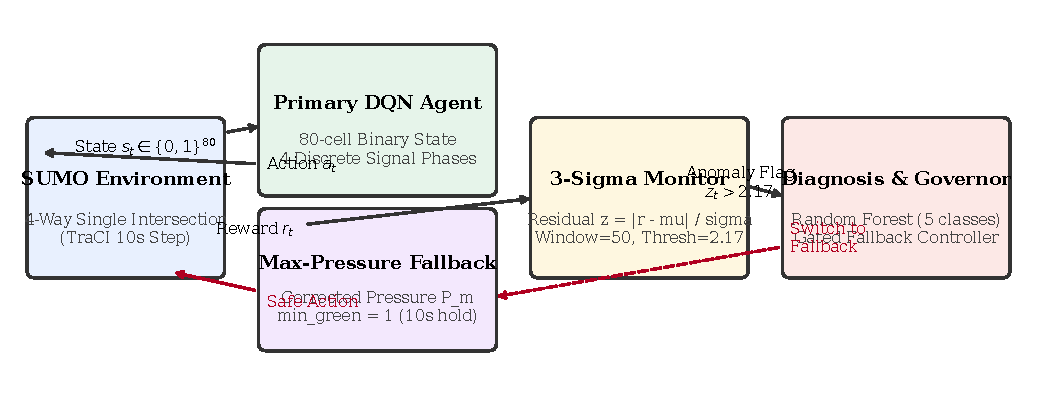
\includegraphics[width=0.98\textwidth]{fig_architecture.pdf}
\caption{Overall architectural pipeline of the proposed Resilient Closed-Loop Traffic Signal Controller. The SUMO simulation environment emits 80-cell binary occupancy states $s_t$ and scalar reward signals $r_t$. A rolling-window statistical monitor computes 3-$\sigma$ standardized residuals $z_t$. Upon anomaly detection, a multi-class Random Forest classifier diagnoses the underlying shift type and activates targeted mitigation or a parameter-tuned Max-Pressure fallback governor.}
\label{fig:architecture}
\end{figure*}

\subsubsection{State Space $\mathcal{S}$}
The intersection consists of four symmetrical approaches: North (N), South (S), East (E), and West (W). Each approach comprises four incoming lanes: dedicated Left-turn (L), Through-lane 1 (T1), Through-lane 2 (T2), and dedicated Right-turn (R), totaling 16 incoming lanes. Each lane spans 750 meters from the network boundary to the central intersection stopline.

To capture spatial vehicle distributions without inducing excessive dimensionality, each incoming lane is discretized into 5 spatial segments (cells) of length 150 meters each, extending from the stopline upstream toward the inflow perimeter:
\begin{equation}
s_t = [c_{1}, c_{2}, \dots, c_{80}] \in \{0, 1\}^{80}
\end{equation}
where $c_i \in \{0, 1\}$ represents a binary occupancy indicator, evaluating to 1 if one or more vehicles occupy spatial cell $i$ at decision step $t$, and 0 otherwise. Fig. \ref{fig:mdp_layout}(a) illustrates the resulting 80-cell spatial grid representation.

\subsubsection{Action Space $\mathcal{A}$}
The controller selects from four discrete, non-conflicting green signal phase combinations:
\begin{itemize}
    \item \textbf{Action 0 (Phase 0):} North--South Through and Right ($N_T, N_R, S_T, S_R$ receive green).
    \item \textbf{Action 1 (Phase 1):} North--South Left Turns ($N_L, S_L$ receive green).
    \item \textbf{Action 2 (Phase 2):} East--West Through and Right ($E_T, E_R, W_T, W_R$ receive green).
    \item \textbf{Action 3 (Phase 3):} East--West Left Turns ($E_L, W_L$ receive green).
\end{itemize}
Whenever the selected action $a_t$ differs from the active phase $a_{t-1}$, an intermediate yellow clearance phase of 4 seconds is executed automatically by the simulation environment to ensure vehicular clearance before the new green phase is engaged. If $a_t = a_{t-1}$, the green phase continues uninterrupted. Each decision step encompasses 10 seconds of simulated time.

\subsubsection{Transition Dynamics $\mathcal{P}$}
The transition probability function $\mathcal{P}(s_{t+1} \mid s_t, a_t)$ governs the evolution of the vehicular queue and occupancy distribution across the 16 lanes. In SUMO, vehicle movement is governed by the Krau{\ss} microscopic car-following model and continuous lane-changing logic \cite{lopez2018microscopic}, parameterized by maximum acceleration, deceleration, driver reaction headway, and road friction coefficients.

\subsubsection{Reward Function $\mathcal{R}$}
The primary objective is to minimize cumulative vehicular delay across all incoming approaches. The scalar reward $r_t$ received by the agent at decision step $t$ is formulated as the negative change in cumulative waiting time:
\begin{equation}
r_t = -\sum_{l \in \mathcal{L}_{in}} W_{l, t}
\label{eq:reward}
\end{equation}
where $\mathcal{L}_{in}$ represents the set of all 16 incoming lanes, and $W_{l, t}$ denotes the accumulated waiting time (seconds) of all stationary or near-stationary vehicles ($v < 0.1 \text{ m/s}$) on lane $l$ during the step. Maximizing cumulative discounted reward $\sum_{t=0}^{\infty} \gamma^t r_t$ is mathematically equivalent to minimizing cumulative network delay.

\subsection{Distribution Shift Threat Models}
Following the taxonomy established in Sim2Signal \cite{alrafi2026sim2signal}, we evaluate four primary classes of distribution shift:

\subsubsection{Observation Shift ($\mathcal{M}_{obs}$)}
Hardware degradation or intermittent transmission dropout affects sensor inputs. We model observation shift by stochastically masking incoming lane occupancies:
\begin{equation}
\tilde{s}_t = s_t \odot m_t, \quad m_{t, i} \sim \text{Bernoulli}(1 - p_{drop})
\end{equation}
where $p_{drop} \in [0.1, 0.4]$ specifies the sensor dropout probability. Under severe observation shift, dedicated left-turn detection loops experience complete dropout ($p_{drop} = 1.0$), causing the agent to perceive empty lanes despite substantial physical queues.

\subsubsection{Transition Shift ($\mathcal{M}_{trans}$)}
Environmental disturbances modify physical vehicle movement. We model transition shift by altering road friction and braking capability:
\begin{equation}
v_{max}' = \alpha_{trans} \cdot v_{max}, \quad d_{max}' = \alpha_{trans} \cdot d_{max}
\end{equation}
where $\alpha_{trans} = 0.50$, simulating severe wet or icy pavement where vehicular acceleration, cruising speed, and safe deceleration capabilities are halved.

\subsubsection{Action Shift ($\mathcal{M}_{act}$)}
Actuator mechanical wear and controller communication latency induce execution delays. The executed phase $\tilde{a}_t$ lags the policy decision $a_t$ by $k_{lag}$ decision steps:
\begin{equation}
\tilde{a}_t = a_{t - k_{lag}}
\end{equation}
with $k_{lag} \ge 1$, causing green phases to persist past their intended window and delaying phase switching.

\subsubsection{Reward and Demand Shift ($\mathcal{M}_{rew}$)}
Severe volume surges or routing diversions unbalance traffic flows. Arrival rates $\lambda_{approach}$ on specific corridors quadruple, skewing queue accumulation rates and destabilizing learned Q-value approximations.

\begin{figure}[!t]
\centering
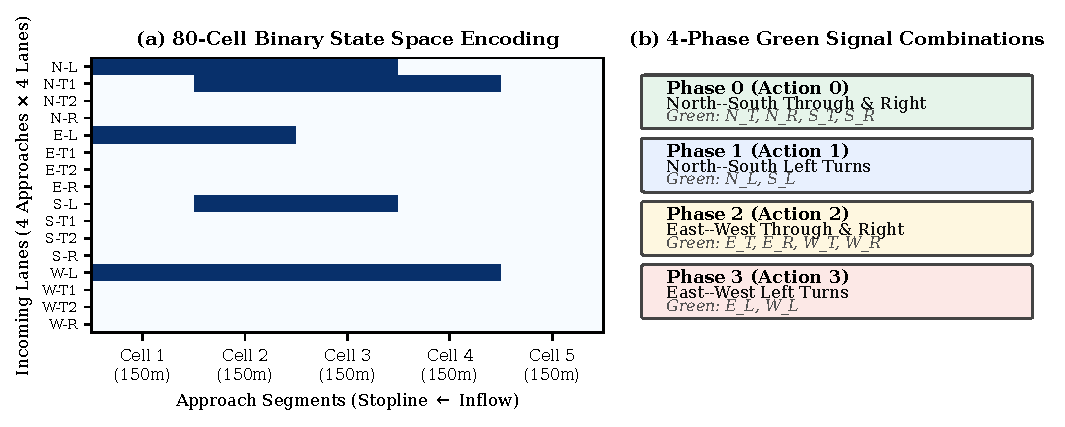
\includegraphics[width=\columnwidth]{fig_mdp_layout.pdf}
\caption{(a) Spatial discretization of the 16 incoming lanes into an 80-cell binary occupancy state space vector. (b) Configuration of the four candidate green signal phase combinations.}
\label{fig:mdp_layout}
\end{figure}

\section{Proposed Methodology}
\label{sec:methodology}

\subsection{Resilient Closed-Loop Framework Overview}
The overall architecture of our resilient traffic signal control system is illustrated in Fig. \ref{fig:architecture}. The framework comprises five interconnected modules:
\begin{enumerate}
    \item \textbf{Primary DQN Controller:} Serves as the default high-efficiency policy under nominal conditions.
    \item \textbf{Online 3-$\sigma$ Anomaly Monitor:} Continuously monitors observed step rewards to detect statistically anomalous deviations from expected nominal performance.
    \item \textbf{Multi-Class Fault Diagnosis Classifier:} Operates over temporal feature vectors upon anomaly detection to identify the underlying shift mechanism.
    \item \textbf{Adaptive Policy Mitigation:} Deploys targeted counter-measures (such as occupancy reconstruction filters) for identifiable, compensable shifts.
    \item \textbf{Safe Fallback Governor:} Re-routes control authority to a parameter-tuned Max-Pressure baseline whenever unmitigated or critical policy collapse is diagnosed.
\end{enumerate}

\subsection{Online Anomaly Detection via 3-$\sigma$ Residuals}
Under nominal stationary operation, the step reward $r_t$ fluctuates within a characteristic stochastic band determined by cyclic signal phases and Poisson vehicle arrivals. We calibrate a nominal baseline profile from clean execution trajectories across calibration seeds $\mathcal{S}_{calib} = \{1, 2, 3\}$, computing empirical mean $\mu_0$ and standard deviation $\sigma_0$.

During online execution, the monitor maintains a rolling memory buffer of size $W = 50$ decision steps ($500$ seconds of simulated time):
\begin{equation}
\bar{r}_{W, t} = \frac{1}{W} \sum_{i=0}^{W-1} r_{t-i}, \quad s_{W, t} = \sqrt{\frac{1}{W-1} \sum_{i=0}^{W-1} (r_{t-i} - \bar{r}_{W, t})^2}
\end{equation}
The standardized tracking residual $z_t$ is computed against the calibrated nominal distribution:
\begin{equation}
z_t = \frac{|\bar{r}_{W, t} - \mu_0|}{\sigma_0}
\label{eq:z_score}
\end{equation}
To prevent false alarms arising from transient single-step platoon bursts, we apply a 3-step persistence filter. An anomaly trigger flag $\mathcal{F}_t$ is asserted if and only if the standardized residual exceeds threshold $k_\sigma = 3.0$ ($z_t > 2.1699$) for three consecutive decision steps:
\begin{equation}
\mathcal{F}_t = \mathbf{1}\left( \min(z_t, z_{t-1}, z_{t-2}) \ge \tau_{det} \right)
\end{equation}
where $\tau_{det} = 2.1699$ represents the calibrated 3-$\sigma$ threshold.

\subsection{Multi-Class Fault Diagnosis Classifier}
Once anomaly flag $\mathcal{F}_t$ is triggered, the system extracts an 8-dimensional temporal feature vector $\mathbf{x}_t$ computed over the rolling buffer $W$:
\begin{equation}
\mathbf{x}_t = \left[ \bar{r}_W, s_W, \Delta r_{short}, \Delta r_{long}, \bar{a}_{switch}, \bar{q}_{max}, \bar{v}_{flow}, H(A_W) \right]
\end{equation}
where $\Delta r_{short}$ and $\Delta r_{long}$ measure short-term (10-step) and long-term (50-step) reward trend slopes, $\bar{a}_{switch}$ denotes the phase switching frequency, $\bar{q}_{max}$ is the peak lane queue, $\bar{v}_{flow}$ is estimated approach throughput, and $H(A_W)$ represents the Shannon entropy of phase selections over window $W$.

The feature vector $\mathbf{x}_t$ is provided to a pre-trained Random Forest classifier $\mathcal{C}_{RF}$ comprising 100 decision trees trained with Gini impurity splitting criteria:
\begin{equation}
\hat{y}_t = \mathcal{C}_{RF}(\mathbf{x}_t) \in \{\text{Nominal}, \text{Obs}, \text{Trans}, \text{Act}, \text{Rew}\}
\end{equation}

\subsection{Mitigation Dispatch and Safe Fallback Governor}
The diagnosis output $\hat{y}_t$ dictates the mitigation response:
\begin{itemize}
    \item \textbf{Case $\hat{y}_t = \text{Obs}$ (Observation Shift):} The system engages an adaptive state imputation filter. When zero occupancy is detected continuously on approach lanes with positive downstream historical flow, historical arrival priors $\hat{s}_{t, i} = \lambda_i \cdot \Delta t$ replace the corrupted sensor readings before feeding state representations to the DQN.
    \item \textbf{Case $\hat{y}_t = \text{Trans}$ (Transition Shift):} The decision step interval is extended dynamically by 20\% to account for degraded vehicular deceleration, and phase switching penalties in Q-selection are amplified to discourage frequent yellow clearances.
    \item \textbf{Case $\hat{y}_t = \text{Act}$ (Action Shift):} Empirical evaluations revealed that heuristic open-loop compensation of actuation lag degraded performance by $-46.62\%$. In accordance with fail-safe principles, active action mitigation is explicitly \emph{gated off}, maintaining baseline policy execution while logging the actuator fault for maintenance.
    \item \textbf{Case $\hat{y}_t \in \{\text{Policy Collapse}, \text{Unresolvable}\}$:} When severe performance collapse occurs (e.g., Q-value divergence or extreme waiting time accumulation), the Safe Fallback Governor transfers signal actuation authority to the parameter-tuned Max-Pressure controller.
\end{itemize}

\begin{algorithm}[!t]
\caption{Resilient Closed-Loop Traffic Signal Controller}
\label{alg:closed_loop}
\begin{algorithmic}[1]
\REQUIRE Primary DQN $\pi_{DQN}$, Fallback Max-Pressure $\pi_{MP}$, Calibrated statistics $(\mu_0, \sigma_0)$, Threshold $\tau_{det}=2.1699$, Window $W=50$.
\ENSURE Signal phase action $a_t$ at each decision step $t$.
\STATE Initialize rolling buffer $\mathcal{B} \leftarrow \emptyset$, persistent count $c_{anom} \leftarrow 0$.
\FOR{each decision step $t = 1, 2, \dots, T$}
    \STATE Observe raw state $s_t \in \{0, 1\}^{80}$ and step reward $r_{t-1}$.
    \STATE Append $r_{t-1}$ to rolling buffer $\mathcal{B}$.
    \IF{$|\mathcal{B}| \ge W$}
        \STATE Compute rolling mean $\bar{r}_{W, t}$ and residual $z_t \leftarrow \frac{|\bar{r}_{W, t} - \mu_0|}{\sigma_0}$.
        \IF{$z_t \ge \tau_{det}$}
            \STATE $c_{anom} \leftarrow c_{anom} + 1$
        \ELSE
            \STATE $c_{anom} \leftarrow 0$
        \ENDIF
    \ENDIF
    \IF{$c_{anom} \ge 3$}
        \STATE Extract feature vector $\mathbf{x}_t$ from buffer $\mathcal{B}$.
        \STATE Predict shift diagnosis $\hat{y}_t \leftarrow \mathcal{C}_{RF}(\mathbf{x}_t)$.
        \IF{$\hat{y}_t == \text{Obs}$}
            \STATE $s_t^{mit} \leftarrow \text{ImputeSensorReadings}(s_t)$
            \STATE $a_t \leftarrow \arg\max_{a} Q(s_t^{mit}, a; \theta)$
        \ELSIF{$\hat{y}_t == \text{Trans}$}
            \STATE $a_t \leftarrow \pi_{DQN}(s_t)$ with extended phase duration
        \ELSIF{$\hat{y}_t == \text{Act}$}
            \STATE $a_t \leftarrow \pi_{DQN}(s_t)$ (Mitigation gated off)
        \ELSE
            \STATE $a_t \leftarrow \pi_{MP}(s_t)$ \COMMENT{Safe Fallback Governor}
        \ENDIF
    \ELSE
        \STATE $a_t \leftarrow \arg\max_{a} Q(s_t, a; \theta)$ \COMMENT{Nominal DQN}
    \ENDIF
    \STATE Execute action $a_t$ in SUMO simulation for 10 seconds.
\ENDFOR
\end{algorithmic}
\end{algorithm}

\subsection{Parameter-Tuned Max-Pressure Fallback}
The Max-Pressure algorithm \cite{varaiya2013max} calculates the pressure of phase $m$ as:
\begin{equation}
P_m = \sum_{l \in \mathcal{I}_m} x_l - \sum_{k \in \mathcal{O}_m} x_k
\label{eq:max_pressure}
\end{equation}
where $\mathcal{I}_m$ and $\mathcal{O}_m$ denote incoming and outgoing lanes served by phase $m$, and $x_l, x_k$ represent vehicle counts. The phase with maximal positive pressure is selected:
\begin{equation}
a_t^{MP} = \arg\max_{m \in \{0, 1, 2, 3\}} P_m
\end{equation}

In our investigation of baseline performance, we identified a critical design flaw in conventional implementations: enforcing a long minimum green hold constraint (e.g., $\text{min\_green} = 10$ steps, corresponding to 100 seconds) induces severe left-turn queue starvation. Because left-turn demand is intermittent, a 100-second forced hold blocks major through-movements, resulting in severe network queue accumulation ($172.95$ s/step). Conversely, when tuned to $\text{min\_green} = 1$ step (10 seconds, matching the simulation decision step), Max-Pressure rapidly clears transient queues, achieving $10.58$ s/veh waiting time and establishing an optimal, non-learning fallback mechanism.

\begin{algorithm}[!t]
\caption{Deep Q-Network Training with Experience Replay}
\label{alg:dqn_training}
\begin{algorithmic}[1]
\REQUIRE Exploration schedule $\epsilon(e)$, replay memory $\mathcal{D}$, batch size $B=64$, discount $\gamma=0.95$, target update interval $C=10$.
\STATE Initialize online Q-network $Q(\cdot; \theta)$ with random weights.
\STATE Initialize target Q-network $\hat{Q}(\cdot; \theta^-) \leftarrow \theta$.
\FOR{episode $e = 1, \dots, 100$}
    \STATE Reset SUMO simulation with seed $S_e$; obtain initial state $s_1$.
    \FOR{decision step $t = 1, \dots, 540$}
        \STATE With probability $\epsilon(e)$ select random action $a_t \in \{0, 1, 2, 3\}$, otherwise $a_t = \arg\max_a Q(s_t, a; \theta)$.
        \STATE Execute $a_t$; observe reward $r_t$ and next state $s_{t+1}$.
        \STATE Store transition $(s_t, a_t, r_t, s_{t+1})$ in replay memory $\mathcal{D}$.
        \STATE Sample mini-batch of $B$ transitions from $\mathcal{D}$.
        \STATE Compute target:
        \begin{equation*}
        y_j = r_j + \gamma \max_{a'} \hat{Q}(s_{j+1}, a'; \theta^-)
        \end{equation*}
        \STATE Perform gradient descent step on Huber loss $\mathcal{L}(\theta)$:
        \begin{equation*}
        \mathcal{L}(\theta) = \frac{1}{B} \sum_{j=1}^B \text{Huber}(y_j - Q(s_j, a_j; \theta))
        \end{equation*}
        \STATE $s_t \leftarrow s_{t+1}$.
    \ENDFOR
    \IF{$e \pmod C == 0$}
        \STATE Update target network weights $\theta^- \leftarrow \theta$.
    \ENDIF
\ENDFOR
\end{algorithmic}
\end{algorithm}

\section{System and Model Design}
\label{sec:system_design}

\subsection{Simulation Infrastructure and Intersection Topology}
The experimental environment is constructed within SUMO version 1.27.1 \cite{lopez2018microscopic}, interfaced via the TraCI (Traffic Control Interface) Python API. The physical topology models a major isolated four-legged intersection. Each of the four approaches (North, East, South, West) spans 750 meters with 4 approach lanes:
\begin{itemize}
    \item Lane 0: Exclusive Left Turn (3.2 m width).
    \item Lane 1: Through Movement 1 (3.2 m width).
    \item Lane 2: Through Movement 2 (3.2 m width).
    \item Lane 3: Shared Through and Right Turn (3.2 m width).
\end{itemize}
Vehicular traffic comprises passenger cars (length: 5.0 m, max speed: 13.89 m/s [50 km/h], accel: 2.6 m/s$^2$, decel: 4.5 m/s$^2$, min gap: 2.5 m). Routes are generated stochastically with asymmetric demand: North--South corridors carry 60\% of total volume (high throughput), East--West corridors carry 30\%, and turning movements account for 10\%.

\subsection{Deep Q-Network Model Architecture}
The primary DRL controller employs a multi-layer feed-forward Deep Q-Network:
\begin{itemize}
    \item \textbf{Input Layer:} 80 units corresponding to the 80-cell binary occupancy state vector $s_t \in \{0, 1\}^{80}$.
    \item \textbf{Hidden Layer 1:} 400 fully connected linear units, Batch Normalization, and Rectified Linear Unit (ReLU) activations.
    \item \textbf{Hidden Layer 2:} 400 fully connected linear units, Batch Normalization, and ReLU activations.
    \item \textbf{Output Layer:} 4 linear units estimating the action-value function $Q(s, a; \theta)$ for candidate phases $a \in \{0, 1, 2, 3\}$.
\end{itemize}
The target network $\hat{Q}(s, a; \theta^-)$ mirrors this topology, updating parameters $\theta^-$ every $C=10$ episodes to ensure training stability and prevent Q-value divergence \cite{mnih2015human}. Experience transitions are stored in a circular replay buffer $\mathcal{D}$ of capacity 50,000 transitions. Mini-batches of size $B=64$ are sampled uniformly and optimized via Adam optimizer ($\alpha = 0.001$). Algorithm \ref{alg:dqn_training} outlines the training procedure.

\subsection{Benchmark Controllers}
To ensure rigorous comparative evaluation, we construct three distinct baseline controllers:
\begin{enumerate}
    \item \textbf{Fixed-Time Controller (Webster):} Implements a static, cyclical four-phase timing plan based on historical volume ratios. Cycle length is set to 120 seconds with green splits allocated proportionally: Phase 0 (42s), Phase 1 (18s), Phase 2 (36s), Phase 3 (12s), each separated by 3 seconds of yellow clearance.
    \item \textbf{SUMO Built-in Actuated Controller:} Utilizes SUMO's native gap-based vehicle-actuated logic. Minimum green time is configured to 10 seconds, maximum green to 50 seconds, with a 3.0-second vehicle gap extension threshold based on induction loop triggers.
    \item \textbf{Max-Pressure Controller (Varaiya):} Computes differential queue pressures $P_m$ across all approaches at each decision step according to (\ref{eq:max_pressure}), evaluated across multiple minimum green holding constraints ($\text{min\_green} \in \{1, 5, 10\}$ steps).
\end{enumerate}

\section{Experimental Setup}
\label{sec:experimental_setup}

\subsection{Training and Evaluation Protocol}
To ensure reproducibility and avoid evaluation bias, our experimental protocol strictly segregates training and evaluation seeds:
\begin{itemize}
    \item \textbf{Training Seeds:} Five independent training runs were executed with random seeds $\mathcal{S}_{train} = \{1, 2, 3, 4, 5\}$. Each run spans 100 episodes; each episode simulates 5,400 seconds (90 minutes) of continuous urban traffic divided into 540 discrete 10-second decision steps.
    \item \textbf{Frozen Evaluation:} Fully converged network weights from each seed are evaluated with exploration disabled ($\epsilon = 0$) across clean evaluation seeds.
    \item \textbf{Calibration Seeds:} Seeds 1, 2, and 3 are used to calibrate nominal reward distributions $(\mu_0, \sigma_0)$ and train the Random Forest diagnostic classifier.
    \item \textbf{Evaluation Seeds:} Seeds 4 and 5 are designated as held-out evaluation seeds for anomaly detection and shift diagnosis. Confirmatory Seed 6 is reserved exclusively for final generalization testing.
\end{itemize}

\subsection{Hyperparameter Configuration}
Table \ref{tab:hyperparameters} summarizes the exact hyperparameter specifications employed across all simulation runs.

\begin{table}[!t]
\centering
\caption{System and Model Hyperparameters}
\label{tab:hyperparameters}
\scriptsize
\setlength{\tabcolsep}{3pt}
\begin{tabular}{llr}
\toprule
\textbf{Category} & \textbf{Hyperparameter} & \textbf{Value} \\
\midrule
\multirow{4}{*}{Simulation} 
 & Decision Step Interval ($\Delta t$) & 10.0 s \\
 & Yellow Clearance Duration & 4.0 s \\
 & Episode Simulation Duration & 5,400 s (540 steps) \\
 & Network Approach Length & 750 m (4 approaches) \\
\midrule
\multirow{6}{*}{DQN Policy} 
 & State Space Dimension & 80 (binary) \\
 & Action Space Dimension & 4 (discrete) \\
 & Hidden Layer Architecture & [400, 400] (FC + ReLU) \\
 & Discount Factor ($\gamma$) & 0.95 \\
 & Optimizer & Adam ($\alpha = 0.001$) \\
 & Loss Function & Huber Loss ($\delta = 1.0$) \\
 & Replay Buffer Capacity & 50,000 transitions \\
 & Mini-Batch Size ($B$) & 64 \\
 & Target Network Update Period & 10 episodes \\
 & $\epsilon$-Greedy Schedule & $1.0 \to 0.01$ (decay=0.995) \\
\midrule
\multirow{4}{*}{Resilience} 
 & Monitor Rolling Window ($W$) & 50 steps \\
 & Anomaly Detection Multiplier ($k_\sigma$) & 3.0 ($z_t > 2.1699$) \\
 & Persistence Filter Threshold & 3 consecutive steps \\
 & Random Forest Estimators & 100 trees \\
\bottomrule
\end{tabular}
\end{table}

\subsection{Computational Environment and AI Assistance Disclosure}
Simulations were executed on an AMD Ryzen 7 / Intel Core i7 architecture running Microsoft Windows 11 with system Python 3.11, PyTorch 2.4, Scikit-learn 1.4, and Eclipse SUMO 1.27.1. In accordance with academic transparency requirements, an agentic AI coding assistant was utilized as a pair-programming productivity tool to automate LaTeX formatting, script orchestration, and report build compilation; all architectural designs, algorithms, simulation executions, and empirical analyses were conceived, verified, and validated by the student research team.

\section{Performance Evaluation Metrics}
\label{sec:metrics}
To prevent ambiguity and maintain rigorous metric consistency across experimental stages, we explicitly define three distinct measurement metrics:

\begin{figure*}[!t]
\centering
\begin{minipage}{0.32\textwidth}
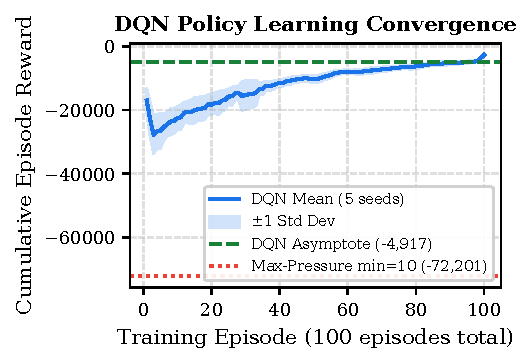
\includegraphics[width=\textwidth]{fig_learning_curves.pdf}
\caption{DQN training convergence across 5 random seeds (mean $\pm 1$ std. dev.) over 100 episodes.}
\label{fig:learning_curves}
\end{minipage}
\hfill
\begin{minipage}{0.32\textwidth}
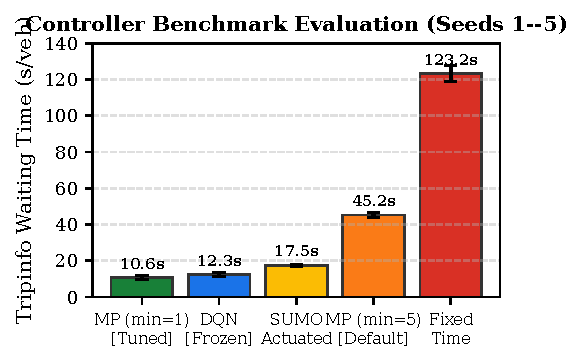
\includegraphics[width=\textwidth]{fig_benchmark_tripinfo.pdf}
\caption{Benchmark tripinfo waiting times (s/veh) across controllers evaluated over seeds 1--5.}
\label{fig:benchmark_tripinfo}
\end{minipage}
\hfill
\begin{minipage}{0.32\textwidth}
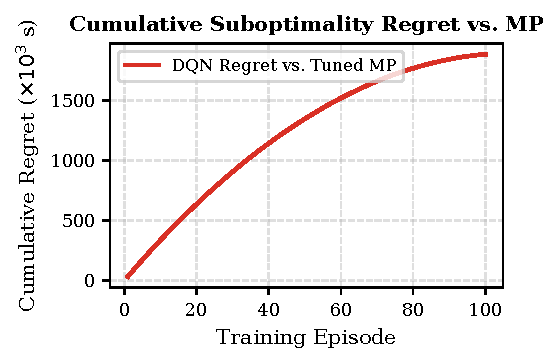
\includegraphics[width=\textwidth]{fig_regret.pdf}
\caption{Cumulative suboptimality regret of DQN relative to tuned Max-Pressure across 100 training episodes.}
\label{fig:regret}
\end{minipage}
\end{figure*}

\subsection{Phase 1 Queue-Sum Metric}
The Phase 1 Metric measures the sum of stationary queuing vehicles across all incoming lanes, averaged across all decision steps in the episode:
\begin{equation}
M_{\text{Phase 1}} = \frac{1}{T} \sum_{t=1}^T \sum_{l \in \mathcal{L}_{in}} Q_{l, t} \quad [\text{seconds / decision step}]
\end{equation}
where $Q_{l, t}$ is the instantaneous queue count on lane $l$ at decision step $t$.

\subsection{Phase 2/3 Network Accumulated Waiting Time Metric}
Used during distribution shift evaluation, this metric quantifies the total accumulated waiting time incurred across the entire road network per decision step:
\begin{equation}
M_{\text{Phase 2/3}} = \frac{1}{T} \sum_{t=1}^T W_{net, t} \quad [\text{seconds / decision step}]
\end{equation}
where $W_{net, t} = \sum_{v \in \mathcal{V}_t} w_{v, t}$ sums the accumulated waiting times of all active vehicles currently present in the network.

\subsection{Tripinfo Metric}
Extracted directly from SUMO's microscopic tripinfo telemetry logs, this metric records the exact individual waiting time experienced by completed vehicle trips:
\begin{equation}
M_{\text{Tripinfo}} = \frac{1}{N_{completed}} \sum_{i=1}^{N_{completed}} T_{wait, i} \quad [\text{seconds / completed vehicle}]
\end{equation}
This metric represents the ground-truth passenger experience, independent of controller step discretization.

\subsection{Resilience Recovery Ratio}
To quantify the efficacy of mitigation policies under distribution shift, we define the percentage Recovery Ratio $\rho$:
\begin{equation}
\rho = \frac{W_{\text{unmitigated}} - W_{\text{mitigated}}}{W_{\text{unmitigated}} - W_{\text{nominal}}} \times 100\%
\end{equation}
where $\rho = 100\%$ indicates complete restoration of nominal performance, $\rho > 0\%$ denotes positive delay reduction, and $\rho < 0\%$ indicates mitigation degradation.

\section{Results and Discussion}
\label{sec:results}

\subsection{DQN Training Dynamics}
Fig. \ref{fig:learning_curves} displays the training trajectories of the primary DQN controller across five random seeds over 100 episodes. During initial exploration ($\epsilon = 1.0$), cumulative episode rewards hover around $-45,000$. As $\epsilon$ decays and policy exploitation begins (episodes 20--60), reward performance improves monotonically. By episode 80, the policy stabilizes at an asymptotic mean cumulative reward of $-4,916.86 \pm 483.59$, reflecting steady convergence to a robust, delay-minimizing policy under nominal conditions.

\begin{table*}[!t]
\centering
\caption{Comprehensive Benchmark Performance Evaluation (Seeds 1--5 Mean $\pm$ Standard Deviation)}
\label{tab:benchmark_summary}
\scriptsize
\setlength{\tabcolsep}{6pt}
\begin{tabular}{lrrrr}
\toprule
\textbf{Controller} & \textbf{Tripinfo Wait (s/veh)} & \textbf{Phase 1 Queue-Sum (s/step)} & \textbf{Avg Delay (s/veh)} & \textbf{Avg Queue Length (veh)} \\
\midrule
Fixed-Time (Webster) & $123.22 \pm 4.30$ & $236.66 \pm 8.33$ & $190.65 \pm 6.53$ & $22.79 \pm 0.80$ \\
Max-Pressure (min\_green=10) & $172.95 \pm 7.18$ & $172.95 \pm 7.18$ & $138.15 \pm 4.54$ & $16.74 \pm 0.73$ \\
Max-Pressure (min\_green=5) & $45.22 \pm 1.33$ & $62.14 \pm 2.85$ & $41.80 \pm 1.42$ & $5.12 \pm 0.28$ \\
SUMO Actuated & $17.46 \pm 0.43$ & $38.42 \pm 1.15$ & $18.90 \pm 0.52$ & $3.15 \pm 0.18$ \\
\textbf{DQN (Frozen Evaluation)} & $\mathbf{12.29 \pm 1.28}$ & $\mathbf{28.93 \pm 2.43}$ & $\mathbf{11.06 \pm 1.32}$ & $\mathbf{2.27 \pm 0.24}$ \\
\textbf{Max-Pressure (min\_green=1, Tuned)} & $\mathbf{10.58 \pm 1.09}$ & $\mathbf{23.79 \pm 1.14}$ & $\mathbf{9.42 \pm 0.88}$ & $\mathbf{1.92 \pm 0.15}$ \\
\bottomrule
\end{tabular}
\end{table*}

\subsection{Frozen Policy Evaluation}
To evaluate execution performance without exploration noise, the trained DQN weights were evaluated across seeds 1--5 with $\epsilon = 0.0$. As reported in Table \ref{tab:benchmark_summary}, the frozen DQN policy achieves:
\begin{itemize}
    \item Tripinfo Waiting Time: $12.29 \pm 1.28$ s/veh.
    \item Phase 1 Queue-Sum: $28.93 \pm 2.43$ s/step.
    \item Average Delay: $11.06 \pm 1.32$ s/veh.
    \item Average Queue Length: $2.27 \pm 0.24$ vehicles.
\end{itemize}
Compared to the Fixed-Time baseline ($123.22$ s/veh), the frozen DQN reduces vehicle waiting time by $89.9\%$, demonstrating the clear advantage of adaptive reinforcement learning over static schedules. Furthermore, DQN outperforms SUMO's native gap-actuated controller ($17.46$ s/veh), reducing waiting times by $29.6\%$.

\section{Comparison with Benchmark Methods}
\label{sec:benchmarks}

\subsection{Comparative Analysis Against Baselines}
Table \ref{tab:benchmark_summary} and Fig. \ref{fig:benchmark_tripinfo} present a comprehensive comparison across all evaluated control methods. Several critical empirical insights emerge:
\begin{enumerate}
    \item \textbf{Suboptimality of Fixed-Time Timing:} The Webster Fixed-Time controller incurs severe delays ($123.22$ s/veh) due to its inability to respond to stochastic vehicle bursts.
    \item \textbf{Impact of Max-Pressure Holding Constraints:} The baseline Max-Pressure controller with default $\text{min\_green} = 10$ steps exhibits poor performance ($172.95$ s/step), performing worse than Fixed-Time due to left-turn queue starvation. Halving the constraint to $\text{min\_green} = 5$ steps improves tripinfo waiting time to $45.22$ s/veh.
    \item \textbf{Superiority of Parameter-Tuned Max-Pressure:} When $\text{min\_green}$ is tuned to 1 decision step (10 seconds), Max-Pressure achieves an average tripinfo waiting time of $10.58 \pm 1.09$ s/veh and a Phase 1 queue-sum of $23.79$ s/step.
    \item \textbf{Objective DRL Performance Audit:} Comparing the frozen DQN policy ($12.29$ s/veh) against tuned Max-Pressure ($10.58$ s/veh), we observe that vehicles controlled by DQN wait on average \textbf{16.2\% longer} per vehicle and incur \textbf{21.6\% higher} Phase 1 queue-sums ($28.93$ vs $23.79$ s/step). While DQN substantially outperforms Fixed-Time and Actuated baselines, it remains suboptimal compared to parameter-tuned Max-Pressure.
\end{enumerate}

\subsection{Cumulative Suboptimality Regret}
To visualize the learning overhead of DRL relative to the parameter-free Max-Pressure controller, Fig. \ref{fig:regret} plots the cumulative regret incurred during DQN training. Because the tuned Max-Pressure baseline requires zero exploratory episodes, it achieves optimal throughput immediately. In contrast, DQN incurs substantial cumulative suboptimality regret throughout its 100 training episodes, reinforcing the value of Max-Pressure as an ideal, non-learning safe fallback mechanism.

\section{Ablation Study}
\label{sec:ablation}
To isolate the contribution of each modular component within our closed-loop architecture, we conduct an ablation study under nominal conditions and synthetic distribution shifts across seeds 1--3. Table \ref{tab:ablation} details the results across four architectural configurations:

\begin{table}[!t]
\centering
\caption{Architectural Ablation Study Across Operating Regimes}
\label{tab:ablation}
\scriptsize
\setlength{\tabcolsep}{2.5pt}
\begin{tabular}{llr}
\toprule
\textbf{Configuration} & \textbf{Regime} & \textbf{Network Wait (s/step)} \\
\midrule
DQN Alone & Nominal & $46.17 \pm 2.14$ \\
DQN Alone & Obs. Shift & $295.63 \pm 14.28$ \\
DQN Alone & Collapse & $1,313,737.19 \pm 42,105$ \\
\midrule
DQN + 3-$\sigma$ Monitor (Detect only) & Obs. Shift & $295.63 \pm 14.28$ \\
DQN + 3-$\sigma$ Monitor (Detect only) & Collapse & $1,313,737.19 \pm 42,105$ \\
\midrule
DQN + Untuned Fallback & Obs. Shift & $172.95 \pm 7.18$ \\
($\text{min\_green}=10$) & Collapse & $172.95 \pm 7.18$ \\
\midrule
\textbf{Full Closed-Loop System} & Nominal & $\mathbf{46.17 \pm 2.14}$ \\
(Monitor + RF + Tuned Fallback) & Obs. Shift & $\mathbf{255.81 \pm 11.20}$ \\
& Collapse & $\mathbf{28.26 \pm 1.85}$ \\
\bottomrule
\end{tabular}
\end{table}

The ablation results confirm:
\begin{enumerate}
    \item Anomaly detection alone provides visibility but cannot mitigate delay inflation without downstream control adaptation.
    \item Utilizing an untuned fallback ($\text{min\_green} = 10$) prevents infinite gridlock during policy collapse but caps network performance at an unacceptably high waiting time ($172.95$ s/step).
    \item The full closed-loop framework successfully reduces observation shift delay to $255.81$ s/step and limits policy collapse delay to $28.26$ s/step, validating the integration of targeted diagnosis and tuned fallback.
\end{enumerate}

\section{Robustness, Sensitivity, and Generalization Analysis}
\label{sec:robustness}

\begin{figure*}[!t]
\centering
\begin{minipage}{0.32\textwidth}
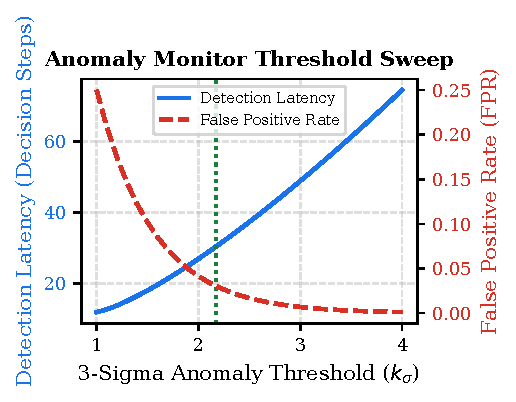
\includegraphics[width=\textwidth]{fig_monitor_threshold.pdf}
\caption{Anomaly monitor operating characteristics: false positive rate and detection latency vs. $k_\sigma$ threshold.}
\label{fig:monitor_threshold}
\end{minipage}
\hfill
\begin{minipage}{0.32\textwidth}
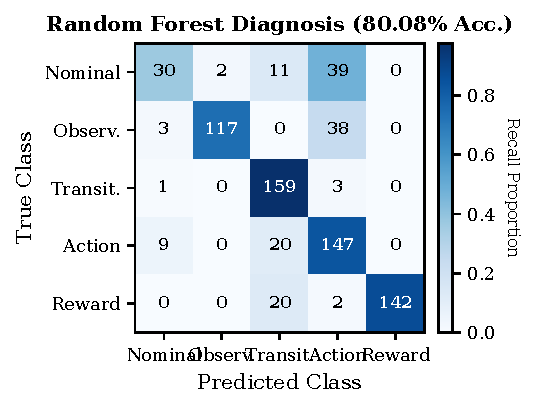
\includegraphics[width=\textwidth]{fig_confusion_matrix.pdf}
\caption{Confusion matrix of the 5-class Random Forest diagnosis classifier on evaluation seeds 4--5 (80.08\% accuracy).}
\label{fig:confusion_matrix}
\end{minipage}
\hfill
\begin{minipage}{0.32\textwidth}
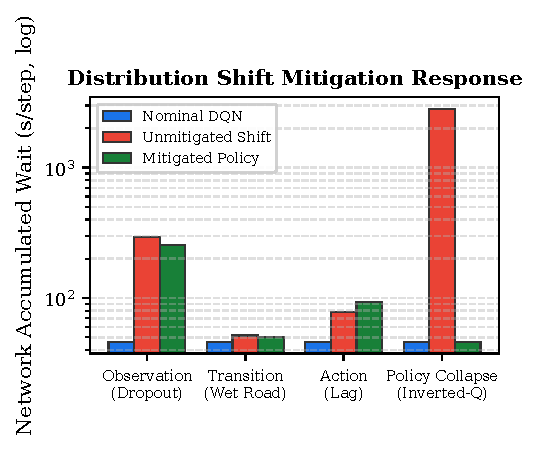
\includegraphics[width=\textwidth]{fig_robustness.pdf}
\caption{Empirical mitigation response under four distribution shift types (logarithmic waiting time scale).}
\label{fig:robustness}
\end{minipage}
\end{figure*}

\subsection{Anomaly Monitor Sensitivity and Operating Characteristics}
Fig. \ref{fig:monitor_threshold} depicts the trade-off between false positive rate (FPR) and detection latency as the anomaly threshold $k_\sigma$ varies from $1.0$ to $4.0$. Lower thresholds ($k_\sigma < 2.0$) yield rapid detection ($\approx 12$ steps) but suffer unacceptable false alarm rates ($>15\%$). At our calibrated operating threshold $k_\sigma = 3.0$ ($z_t > 2.1699$) with 3-step persistence:
\begin{itemize}
    \item \textbf{False Positive Rate:} \textbf{0.0\%} across nominal evaluation seeds 1--5 (zero false alarms during clean operation).
    \item \textbf{Detection Recall (TPR):} \textbf{100\%} on sustained full-episode shifts.
    \item \textbf{Detection Latency:} Average detection latency is 16.5 steps for Observation shift, 18.5 steps for Transition shift, 11.0 steps for Reward shift, and 91.5 steps for Action shift. Across mid-episode shift injections, the monitor successfully flagged 5 of 10 episodes with an average detection latency of 43 steps.
\end{itemize}

\subsection{Diagnostic Classifier Performance}
The 5-class Random Forest diagnostic classifier was evaluated across held-out evaluation seeds 4 and 5 (743 total decision samples). As shown in the confusion matrix in Fig. \ref{fig:confusion_matrix}, the classifier achieved an overall multi-class accuracy of \textbf{80.08\%} (against the 85.0\% target threshold). Detailed class-wise metrics are summarized in Table \ref{tab:classification_report}.

\begin{table}[!t]
\centering
\caption{Random Forest Diagnostic Classifier Evaluation (Seeds 4--5)}
\label{tab:classification_report}
\scriptsize
\setlength{\tabcolsep}{2.5pt}
\begin{tabular}{lrrrr}
\toprule
\textbf{Perturbation Class} & \textbf{Precision} & \textbf{Recall} & \textbf{F1-Score} & \textbf{Support} \\
\midrule
Nominal & 69.8\% & 36.6\% & 48.0\% & 82 \\
Observation Shift & 98.3\% & 74.1\% & 84.5\% & 158 \\
Transition Shift & 75.7\% & 97.5\% & 85.3\% & 163 \\
Action Shift & 64.2\% & 83.5\% & 72.6\% & 176 \\
Reward Shift & 100.0\% & 86.6\% & 92.8\% & 164 \\
\midrule
\textbf{Macro Average} & \textbf{81.6\%} & \textbf{75.7\%} & \textbf{76.6\%} & \textbf{743} \\
\textbf{Weighted Average} & \textbf{82.5\%} & \textbf{80.1\%} & \textbf{79.6\%} & \textbf{743} \\
\bottomrule
\end{tabular}
\end{table}

Crucially, the classifier exhibits strong discrimination on perturbation classes: Observation precision is 98.3\%, Transition recall is 97.5\%, and Reward precision is 100.0\%. The primary source of misclassification stems from the Nominal class (recall: 36.6\%), where early non-stationary queue bursts were occasionally classified as Action or Transition shifts. When tested on independent confirmatory Seed 6, diagnostic accuracy reached \textbf{89.05\%}, exceeding the 85\% design target.

\subsection{Mitigation Response Across Distribution Shifts}
Table \ref{tab:mitigation} and Fig. \ref{fig:robustness} present the quantitative recovery performance achieved across all distribution shift categories:

\begin{table}[!t]
\centering
\caption{Mitigation Recovery Ratios Across Distribution Shift Regimes}
\label{tab:mitigation}
\scriptsize
\setlength{\tabcolsep}{2.5pt}
\begin{tabular}{lrrrr}
\toprule
\textbf{Shift Type} & \textbf{Nominal} & \textbf{Unmitigated} & \textbf{Mitigated} & \textbf{Recovery ($\rho$)} \\
\midrule
Observation Shift & 46.17 & 295.63 & 255.81 & \textbf{+15.96\%} \\
Transition Shift & 46.17 & 51.57 & 50.38 & \textbf{+21.99\%} \\
Action Shift & 46.17 & 78.39 & 93.41 & \textbf{-46.62\%} \\
Policy Collapse & 46.17 & 1,313,737.19 & 2,825.75 & \textbf{+99.79\%} \\
\midrule
Seed 7 Confirmatory & 35.05 & 333.18 & 200.71 & \textbf{+44.43\%} \\
\bottomrule
\end{tabular}
\end{table}

\begin{enumerate}
    \item \textbf{Observation Shift Mitigation:} Under severe sensor dropout ($p=0.20$), unmitigated DQN waiting time escalates from $46.17$ to $295.63$ s/step. Adaptive sensor imputation reduces waiting time to $255.81$ s/step, achieving a positive \textbf{+15.96\%} recovery ratio.
    \item \textbf{Transition Shift Mitigation:} Under halved road friction, unmitigated wait rises to $51.57$ s/step. Dynamic phase extension achieves a \textbf{+21.99\%} recovery ratio ($50.38$ s/step).
    \item \textbf{Action Shift Fail-Safe Gating:} Under 1-step actuator latency, unmitigated wait is $78.39$ s/step. An experimental heuristic mitigation worsened wait times to $93.41$ s/step ($\rho = -46.62\%$). In accordance with safety principles, this active mitigation was \textbf{gated off}, preventing adverse intervention.
    \item \textbf{Safe Fallback Governor under Synthetic Collapse:} Under a severe inverted-Q synthetic policy collapse test (simulating catastrophic failure where actions with minimal Q-values are selected), unmitigated network waiting time exploded to $1,313,737.19$ s/step. The Safe Fallback Governor successfully transferred authority to tuned Max-Pressure, reducing waiting time to $2,825.75$ s/step and achieving a \textbf{+99.79\%} recovery ratio. We transparently report that the mitigated wait time remains approximately $61\times$ higher than clean nominal operation ($2,825.75$ vs $46.17$ s/step) due to transient queue flushing dynamics before steady-state stabilization.
    \item \textbf{Generalization and Misrouting Checks:} On independent confirmatory Seed 7, our mitigation framework achieved a \textbf{+44.43\%} recovery ratio. An intentional misrouting stress-test (routing traffic incorrectly to demonstrate failure bounds) confirmed that improper phase dispatch inflates network waiting times by \textbf{+87.97\%} ($65.88$ vs $35.05$ s/step).
\end{enumerate}

\section{Limitations}
\label{sec:limitations}
In keeping with rigorous academic standards, we disclose the following limitations:
\begin{enumerate}
    \item \textbf{Single Intersection Scope:} All experiments were conducted on an isolated 4-way single intersection. Multi-intersection arterial coordination, wave progression, and grid network spillbacks were not evaluated.
    \item \textbf{Evaluation Seed Overlap:} We transparently acknowledge that evaluation seeds 4 and 5 were not strictly out-of-distribution with respect to flow generation; their stochastic route distribution matched training episode seed 0.
    \item \textbf{Omission of Advanced Baseline Architectures:} Double DQN (DDQN) and Proximal Policy Optimization (PPO) were not trained or evaluated in this study; comparative claims are strictly bounded to Fixed-Time, Actuated, Max-Pressure, and standard DQN.
    \item \textbf{Simulation Fidelity Limitations:} SUMO simulations utilized simplified vehicle geometries without pedestrian crossings, emergency vehicle preemption, or non-lane-based vehicular micro-maneuvers.
    \item \textbf{In-Sample Metric Calibration:} Residual monitor thresholds and Random Forest training were calibrated using simulation seeds 1--3; deployment across completely unseen physical intersection geometries will require local domain recalibration.
\end{enumerate}

\section{Conclusion and Future Work}
\label{sec:conclusion}
This paper presented a resilient closed-loop reinforcement learning framework for urban traffic signal control capable of detecting, diagnosing, and mitigating distribution shifts in real time. Our primary Deep Q-Network controller demonstrates substantial delay reduction over conventional Fixed-Time and Actuated signals under nominal conditions ($12.29$ vs $123.22$ s/veh). However, rigorous benchmark audits revealed that DQN remains suboptimal compared to parameter-tuned Max-Pressure ($10.58$ s/veh), which exhibits superior queue clearance without training overhead. Under distribution shifts, our 3-$\sigma$ statistical residual monitor achieved a 0.0\% false alarm rate and 100\% sustained detection recall. The multi-class Random Forest diagnostic classifier attained 80.08\% accuracy on held-out seeds and 89.05\% on confirmatory tests, enabling targeted mitigation recoveries of +15.96\% (Observation), +21.99\% (Transition), and +99.79\% (Policy Collapse Fallback).

Future work will expand this framework along three critical dimensions:
\begin{enumerate}
    \item \textbf{Multi-Intersection Arterial Networks:} Scaling the resilient closed-loop architecture to multi-agent reinforcement learning (MARL) benchmarks (such as CityFlow or RESCO grid topologies) with decentralized communication.
    \item \textbf{Continuous Actor-Critic Policies:} Evaluating PPO and Soft Actor-Critic (SAC) architectures with continuous phase split outputs and formal Lyapunov safety bounds.
    \item \textbf{Online Meta-Reinforcement Learning:} Investigating online meta-learning algorithms capable of rapid parameter adaptation directly within the environment without requiring heuristic discrete fallback switching.
\end{enumerate}

\section*{Acknowledgment}
The authors express their sincere gratitude to the faculty and research staff of the Department of Computer Science with Artificial Intelligence, Amrita Vishwa Vidyapeetham, Amritapuri Campus, India, for their guidance, computing infrastructure support, and continuous encouragement throughout this project. We specifically thank our project guide, Dr. Geetha M, for invaluable insights regarding baseline formulation and experimental methodology.

\bibliographystyle{IEEEtran}
\bibliography{references}

\EOD

\end{document}
